\chapter{The Large Hadron Collider}
\label{sec:lhcb}

The Large Hadron Collider (LHC) is the most powerfull particle-accelerator on planet earth. With a circumference of $26,7\si{\kilo\metre}$ it is also the longest ring accelerator and it lies between $45\si{\metre}$ and $170\si{\metre}$ below the surface near Geneva in Swizerland. The tunnel was constructed for the LEP experiment between 1984 and 1989 and is operated by the European Organization for Nuclear Research (CERN). The LHC can produce centre of mass energies of $\sqrt{s} = \SI{13}{\tera\electronvolt}$ in proton-proton collisions during Run 2. After the upgrade the LHC will collide particles with the centre of mass energy $\sqrt{s} = \SI{13}{\tera\electronvolt}$.
An image of the accelerators and the experiments is shown in fig. \ref{fig:CERN}\cite{facilityCERN}.

\begin{figure}
  \centering
  \includegraphics[width=0.5\textwidth]{plots/LHC_facility.ppm}
  \caption{an overview of the LHC facilities.}
  \label{fig:CERN}
\end{figure}

By ionizing hydrogen gas, protonsare created and accelerated to $\SI{50}{\mega\electronvolt}$ by the linear accelerator (LINAC 2). Afterwards the beam is injected into the Proton Syncrotron and the Super Proton Synchrotron to a maximum of $\SI{450}{\giga\electronvolt}$ before the beam is brought into the LHC.
The beam containts several bunches with around $\num{1.15e11}$ and a bunch spacing of $\SI{25}{\nano\seconds}$, which is a collision rate of $\SI{40}{\mega\hertz}$.
The LHC houses four major experiments. ATLAS and CMS are classified as general purpose detectors with a detection range of close to $4\pi$. The interaction in these detectors is located in the very center so that tracks going in every direction can possibly be found. Searches for the Higgs Boson is just one of many physics aspects these detectors are build for.
The other two Experiments located at the LHC are ALICE and LHCb.
The ALICE experiment main studies the quark gluon plasma during the runs with lead ion collisions instead of protons.
In this thesis the Scintillating Fibre Tracker (SciFi Tracker) located at the LHCb will be focused at and discussed on the following chapters.

\chapter{The LHCb Experiment\cite{lhcbInfo}}

\begin{figure}
  \centering
  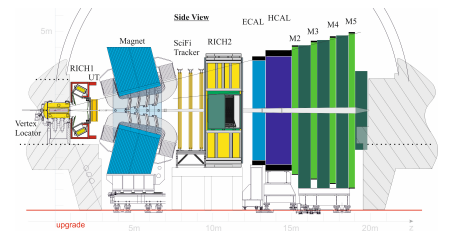
\includegraphics[width=0.5\textwidth]{plots/LHCb_facility.png}
  \caption{a sideview of the LHCb experiment.}
  \label{fig:LHCb}
\end{figure}

The LHCb experiment is a forward spectrometer covering $2 \less \eta \less 5$ in the pseudorapidity range. This experiments main physics goal is beauty quark physics and for high energies, b- and $\bar{b}$-hadrons are heavily produced in a tight forward direction\footnote{They are also produced in a tight backward direction but the experiment is only build for the forward cone.}. A sideview of the LHCb is shown in figure \ref{fig:LHCb}.
The LHCb consists of several smaller detector components namely the Vertex Locator (VELO) right on the intercation point, two Ring Imaging Cherenkov counter (RICH 1 and RICH 2), in front of the spectrometers lies the Trigger Tracker and behind them the SciFi Tracker which is the important part of this thesis. Further back a Scinitllator Pad Detector (SPD) and a Preshower (PS) are mounted followed by the electromagnetic calorimeter and the hadronic calorimeter. In the very back, several muon chambers are mounted for every track that is yet to be determined.

\section{the Scintillating Fibre Tracker}
\label{sec:scifi}
% \begin{enumerate}
%   \item layout
%   \item how does it work?
%   \item what else?
% \end{enumerate}

\chapter{Alignment}
\label{sec:alignment}
martinelli pdf! use some of that information
-> alignment is a minimizing problem (chi2) thats why i looked at chi2 plots

-> global translation and sheering motion don't change chi2 values because residuals are unchanged.

-> weak modes: presence of weak modes affect the convergence (poor, takes many iterations), bias in track parameters.

-> most visible weak modes is the "curvature bias" (sophie has mentioned it sometime. must be on one of my sheets)
also look at twiki!
\section{what is alignment used for?}
short answers:
% \begin{enumerate}
%   \item yielding the best possible reconstruction efficiency
%   \item getting a good feeling for particle masses
%   \item momentum resolution of the detector improved
% \end{enumerate}

for these 3 bullet points i need a subsection explaining it!

\section{when does alignment happen?}
at which point during a run will alignment come into play?

\section{Alignment Methods}

\subsection{using tracks fitted with kalman}
talk pdf. quelle herausfinden!
\subsection{'global' alignment with collision data}
wouter pdf. quelle herausfinden!

\section{Alignment goals}
source for now: DPG2021 pdf exact source will be included!
% \begin{enumerate}
%   \item find the best possible configuration of alignables, degrees of freedom, constraints
%   \item check for weak modes (how? chi2, small eigenvalues)
%   \item null tests as good as possible
%   \item misalignment tests to check alignment
% \end{enumerate}

all of the above is just theory. Now, the story i want to tell starts.
